\chapter{胆道影像解剖}

胆道包括肝内外胆管、胆囊、胆囊管以及胰管等一系列管道结构,它是胆汁和胰液运输至十二指肠的管道,了解正常胆道结构具有十分重要的意义。

\section{检查方法}

诊断胆胰疾病的影像学检查手段有常规X线、超声、CT、血管造影和MRI等,各种检查方法各有其临床使用特点和限度。超声在临床上常作为胆系疾病诊断的首选检查方法,CT与超声相结合能对大多数胆胰疾病作出正确诊断。磁共振水成像技术是近年来磁共振成像重大进展之一,其中以磁共振胆胰管成像(MR
cholangiopancreatography,MRCP)应用最早、最广泛。MRCP自20世纪90年代初德国学者首次提出并应用以来,引起了广泛的关注,是一种发展较快,简便、安全、有效的观察胆胰管系统解剖和诊断胆胰管疾病的影像学检查技术,临床上可作为诊断胆胰管疾病的初筛检查手段。MRCP不需特殊的插管技术,也不必注射造影剂,是一种无创伤性检查,兼有横断面成像和造影检查的长处,既可提供与超声和CT相似的信息,又具有与ERCP类似的造影图像。MRCP与ERCP起着互补的作用,当上消化道手术和改建后,或食管、十二指肠严重狭窄时难以插管,不能作ERCP,这些病例就只能作MRCP检查。MRCP是利用胰液、胆液这些天然的对比剂,通过重建图像后处理,突出含液体的胆胰管结构影像。MRCP技术包括梯度回波(GRE)、快速自旋回波(TSE)以及由其衍化而来的快速采集驰豫增强(RARE)和单次激发快速自旋回波半傅立叶采集序列,采用最大信号强度(MIP)作三维立体重建,可显示胆系全貌,运用工作站中三维成像的连续性和旋转功能可显示胆胰管关系,并可直接观察病变形态,最后结合常规MR图像作出综合诊断。

\section{重建影像}

目前对于胆道最有效的无创成像方法就是MRCP,以下2幅图像即为MRCP图像。由于正常人胰管较细,因此部分正常人的胰管在MRCP上无法显示。
\begin{figure}[!htbp]
 \centering
 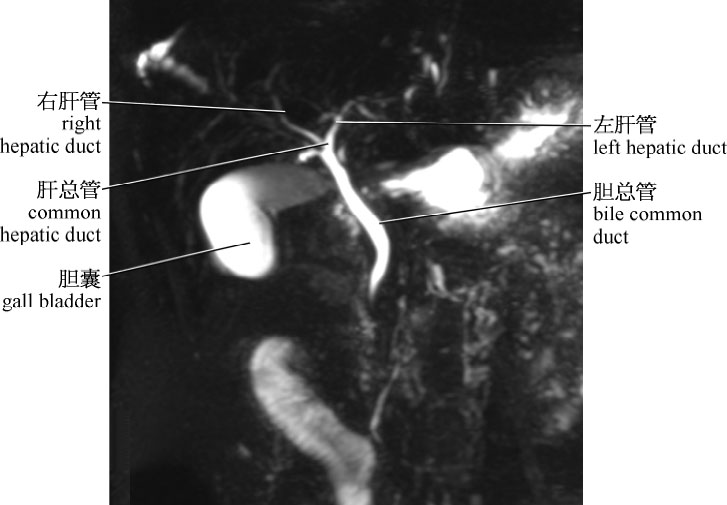
\includegraphics{./images/Image00164.jpg}
  \end{figure} 
 \FloatBarrier

\begin{figure}[!htbp]
 \centering
 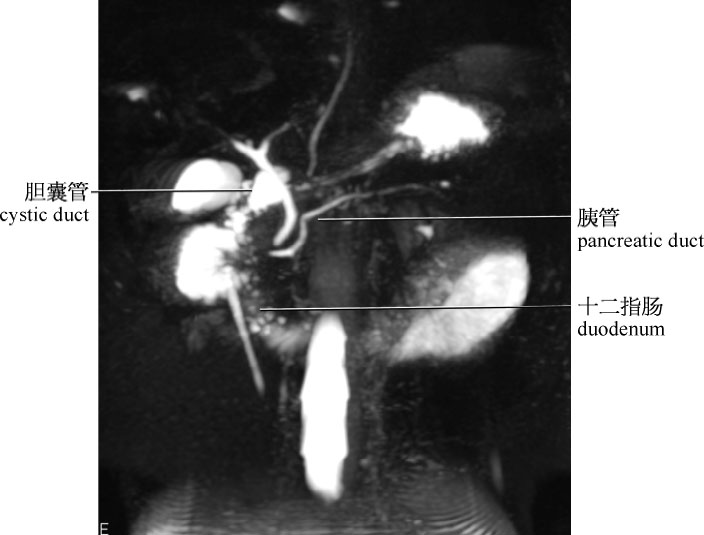
\includegraphics{./images/Image00165.jpg}
  \end{figure} 
 \FloatBarrier

